\section{Synthesis}

\begin{frame}{Problem-specific Knowledge}

\cite{waibel2009genetic} (puck-foraging) and \cite{knudson2010coevolution} ()

\end{frame}

\begin{frame}{Team Genome}
idea: bypass credit-assignment problem altogether by evolving teams as a unit

\begin{itemize}
\item completely clonal group
\begin{itemize}
\item lose out on configuration specialization
\end{itemize}
\item completely non-clonal group
\begin{itemize}
\item too many parameters
\end{itemize}
\item partially clonal group \cite{bongard2000legion}
\begin{itemize}
\item analogy: indirect encoding that exploits symmetries to simplify the genetic search space \cite{bongard2000legion}
\end{itemize}
\item need domain knowledge about team size?
\begin{itemize}
\item not necessarily; evolve team size \cite{bongard2000legion}
\end{itemize}

\end{itemize}

%TODO

\end{frame}

\begin{frame}{Inspiration from Nature}

\begin{columns}
\begin{column}{0.5\textwidth}
hypothesized mechanisms that stabilize cooperation between genetically-dissimilar individuals \cite{vostinar2017suicide, andre2016evolutionary}:
\begin{itemize}
\item transitions of individuality
\item vertical transmission
\item partner selection
\item reciprocity
\end{itemize}
\end{column}
\begin{column}{0.5\textwidth}
\begin{figure}
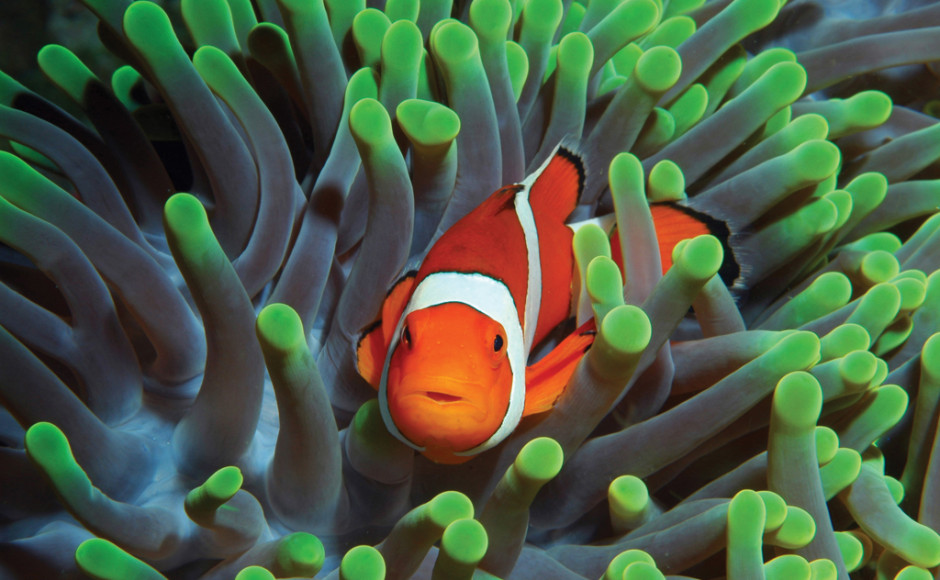
\includegraphics[width=\textwidth]{clownfish}
\caption{
Clownfish and sea anenomones have a symbiotic relationship \cite{dunn1981clownfish}.
}
\label{fig:clownfish}
\end{figure}
\end{column}
\end{columns}
\end{frame}
